\section{Protótipos}
\label{att:proto}

\begin{figure}[h]
\centering
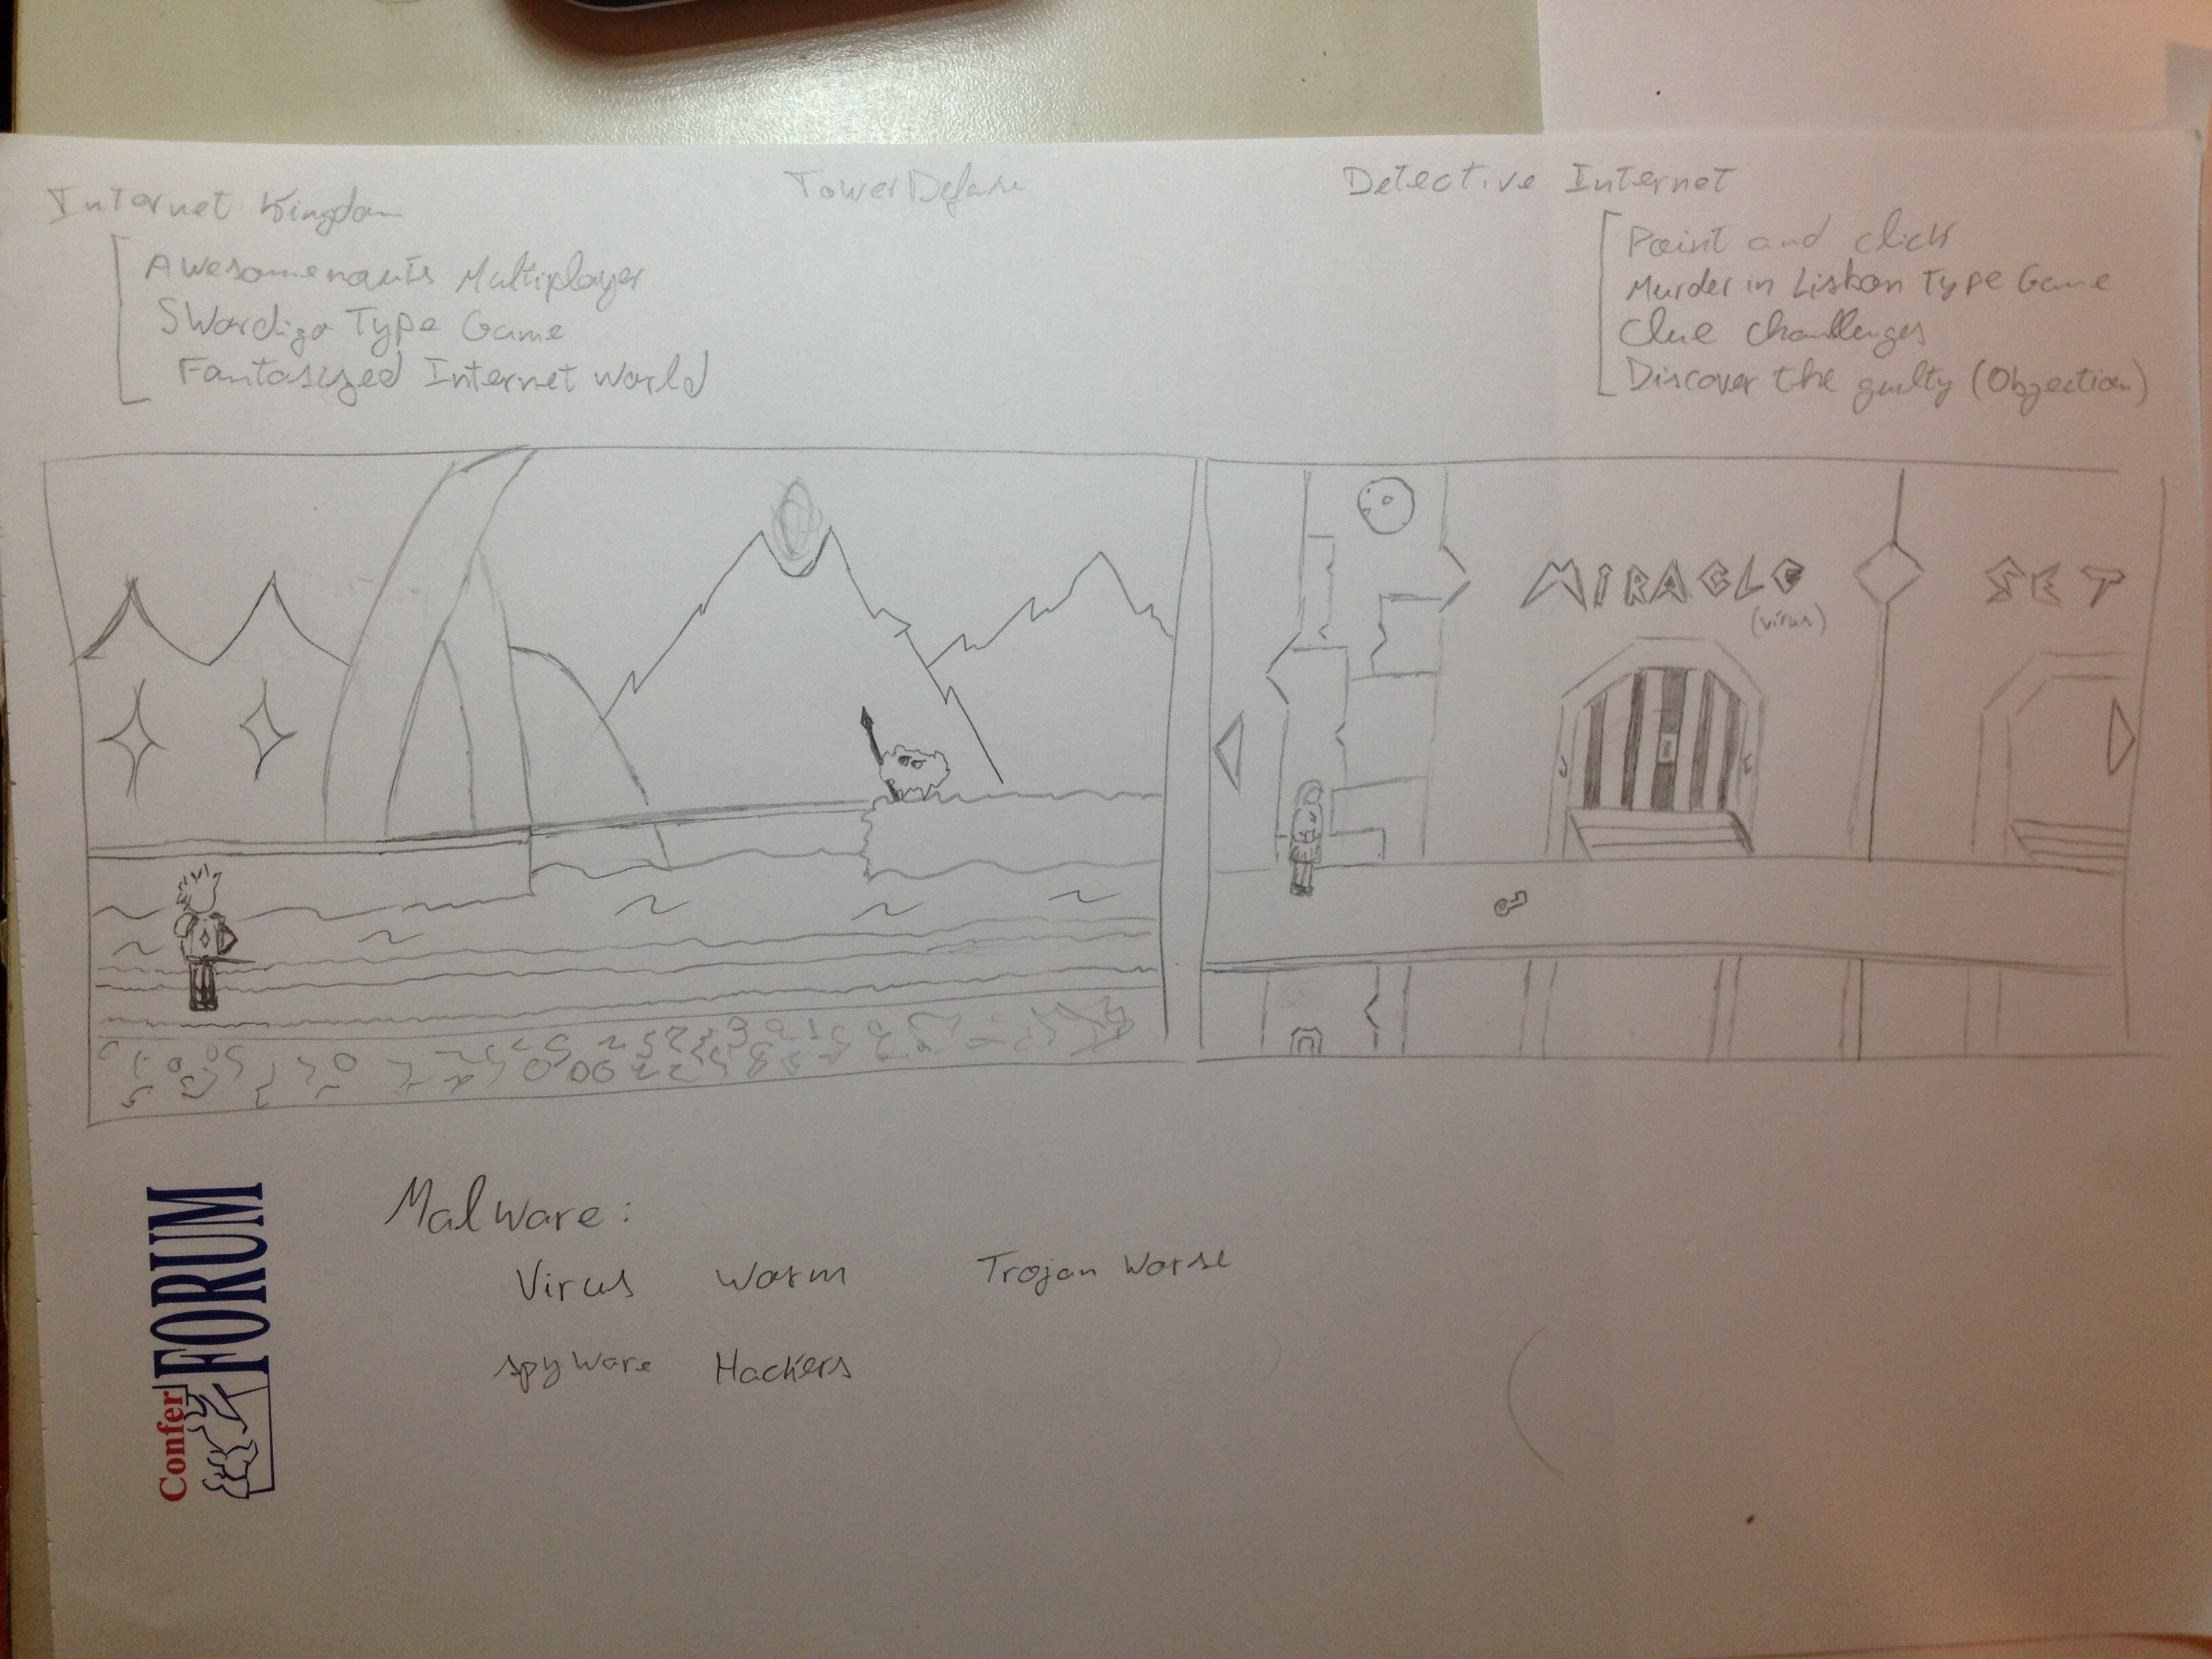
\includegraphics 
	[width = 0.75\textwidth] {Ricardo/ricardo_prototipo_1}
\caption{\label{att:fig:ric:prot1}} Primeiro Protótipo do Ricardo
\end{figure}

\begin{figure}[h]
\centering
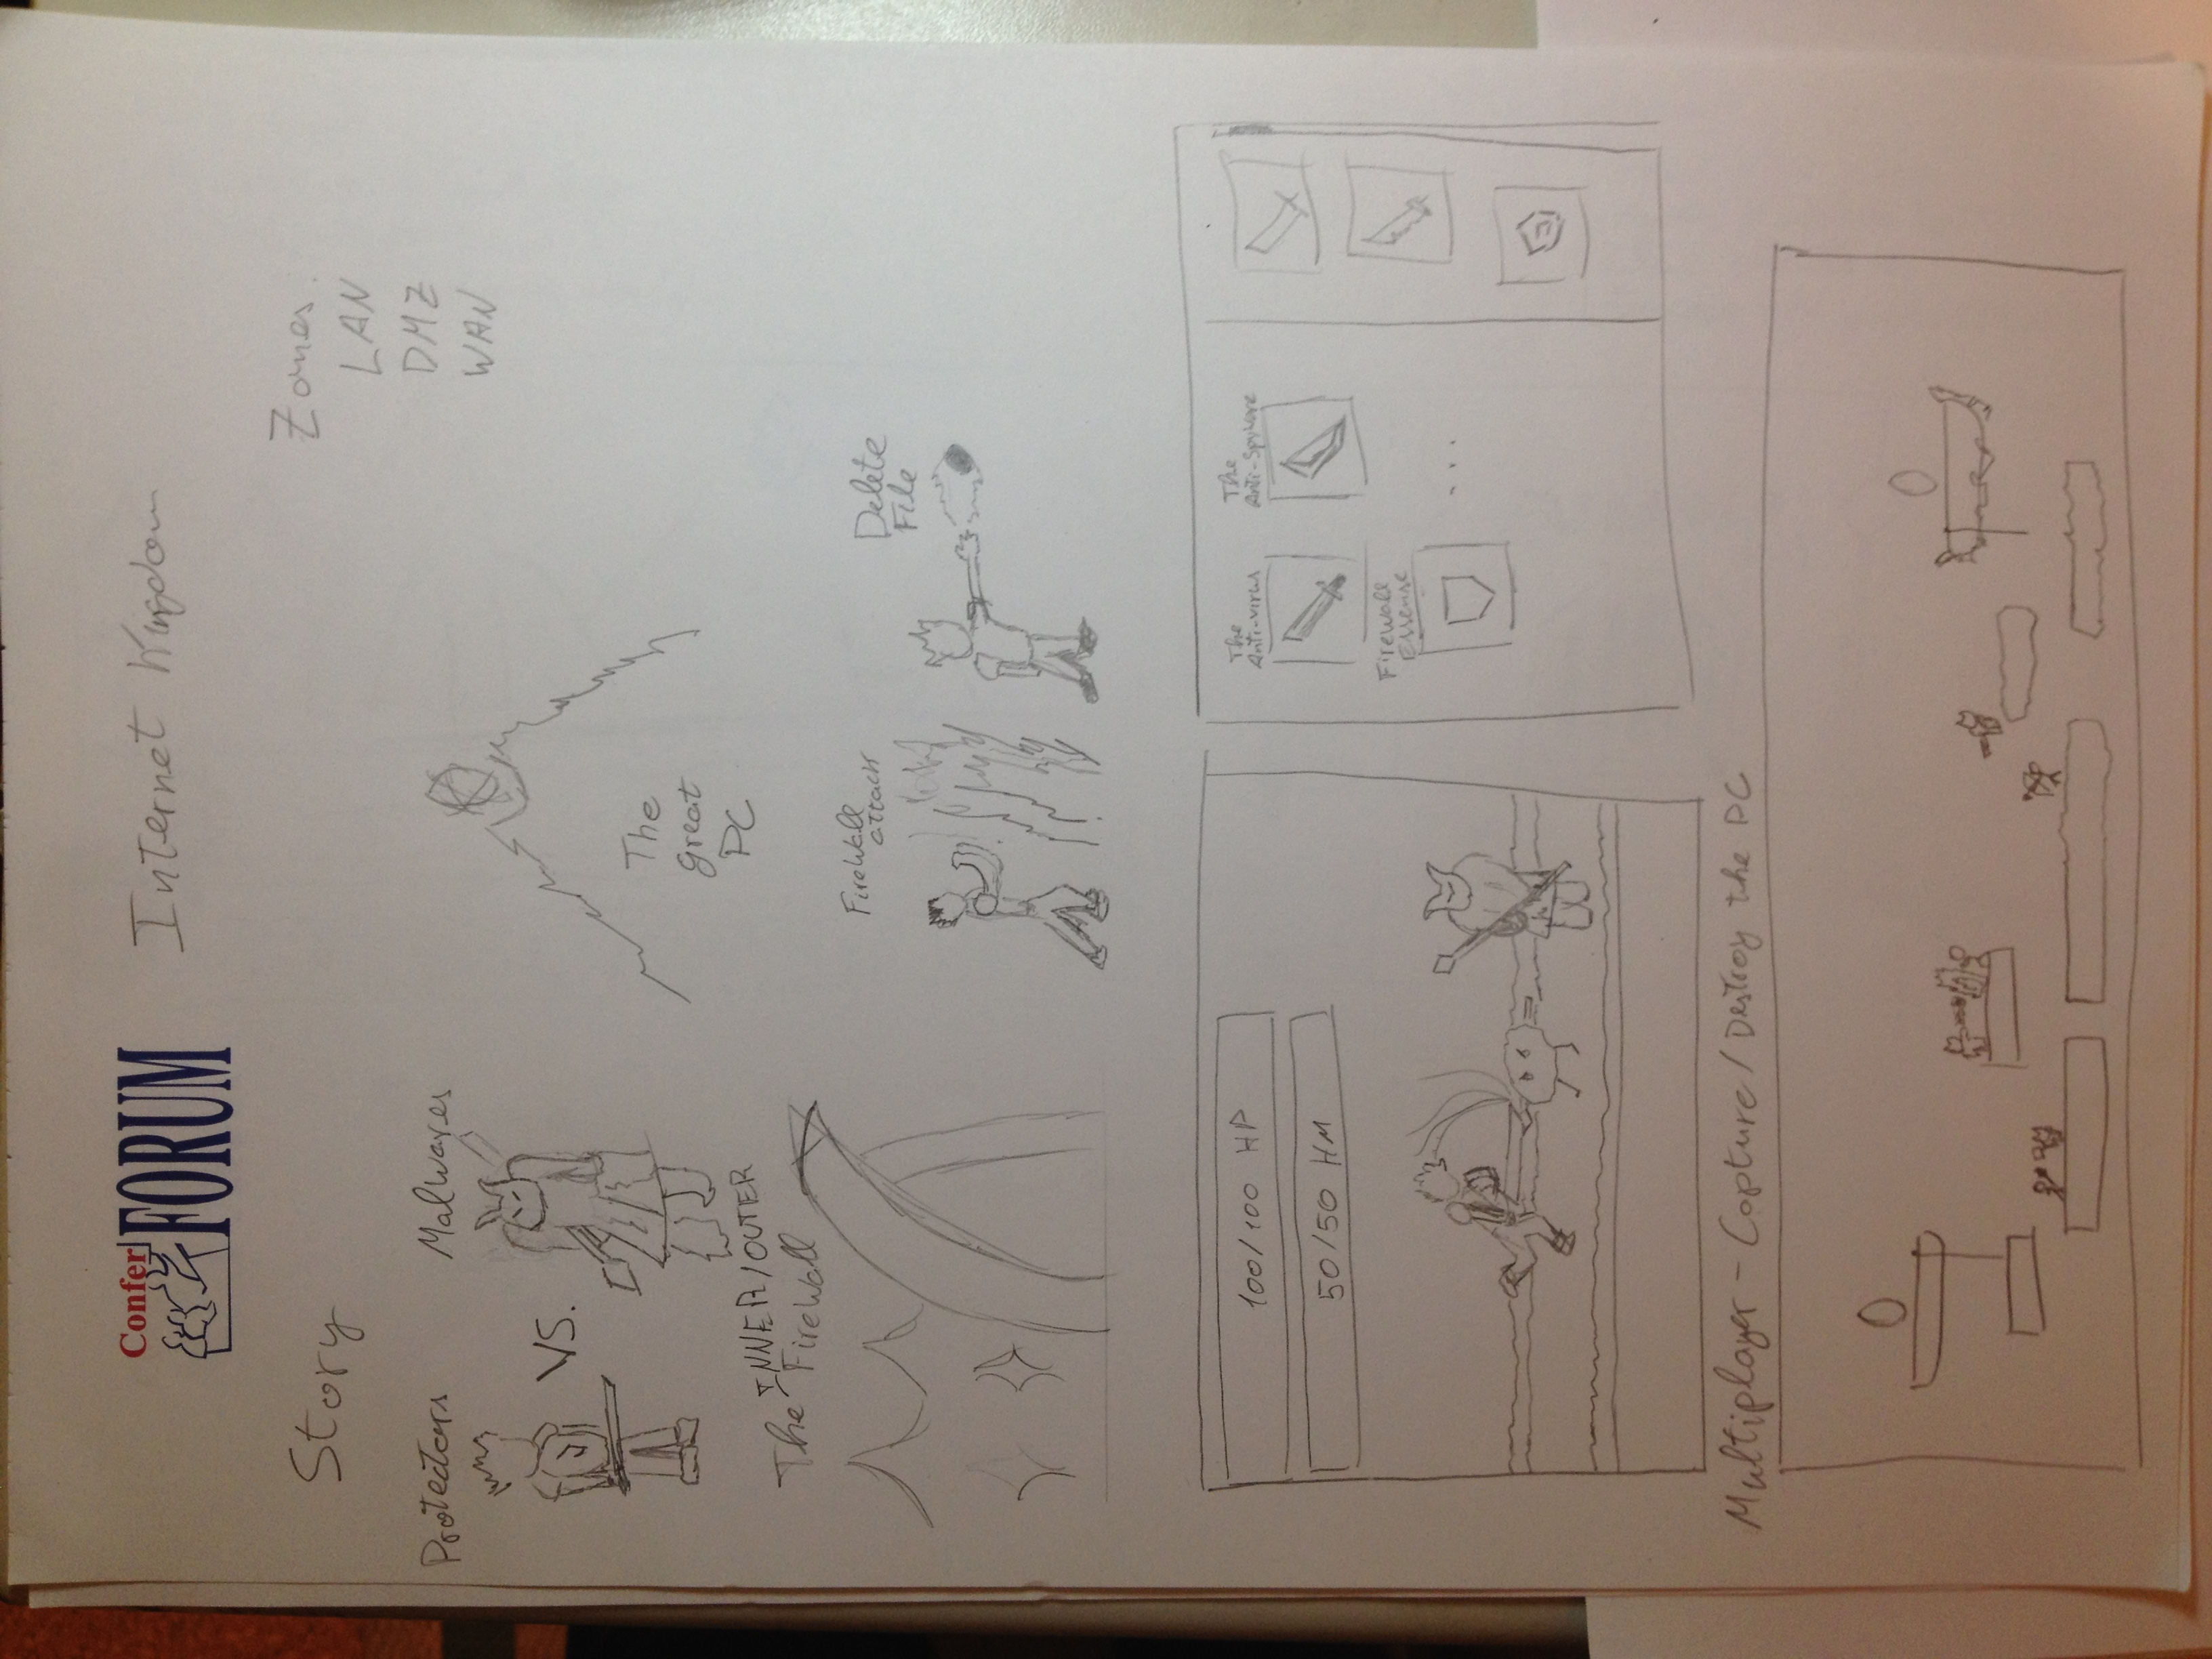
\includegraphics 
	[width = 0.75\textwidth , angle = 270] {Ricardo/ricardo_prototipo_2}
\caption{\label{att:fig:ric:prot2}} Segundo Protótipo do Ricardo
\end{figure}

\begin{figure}[h]
\centering
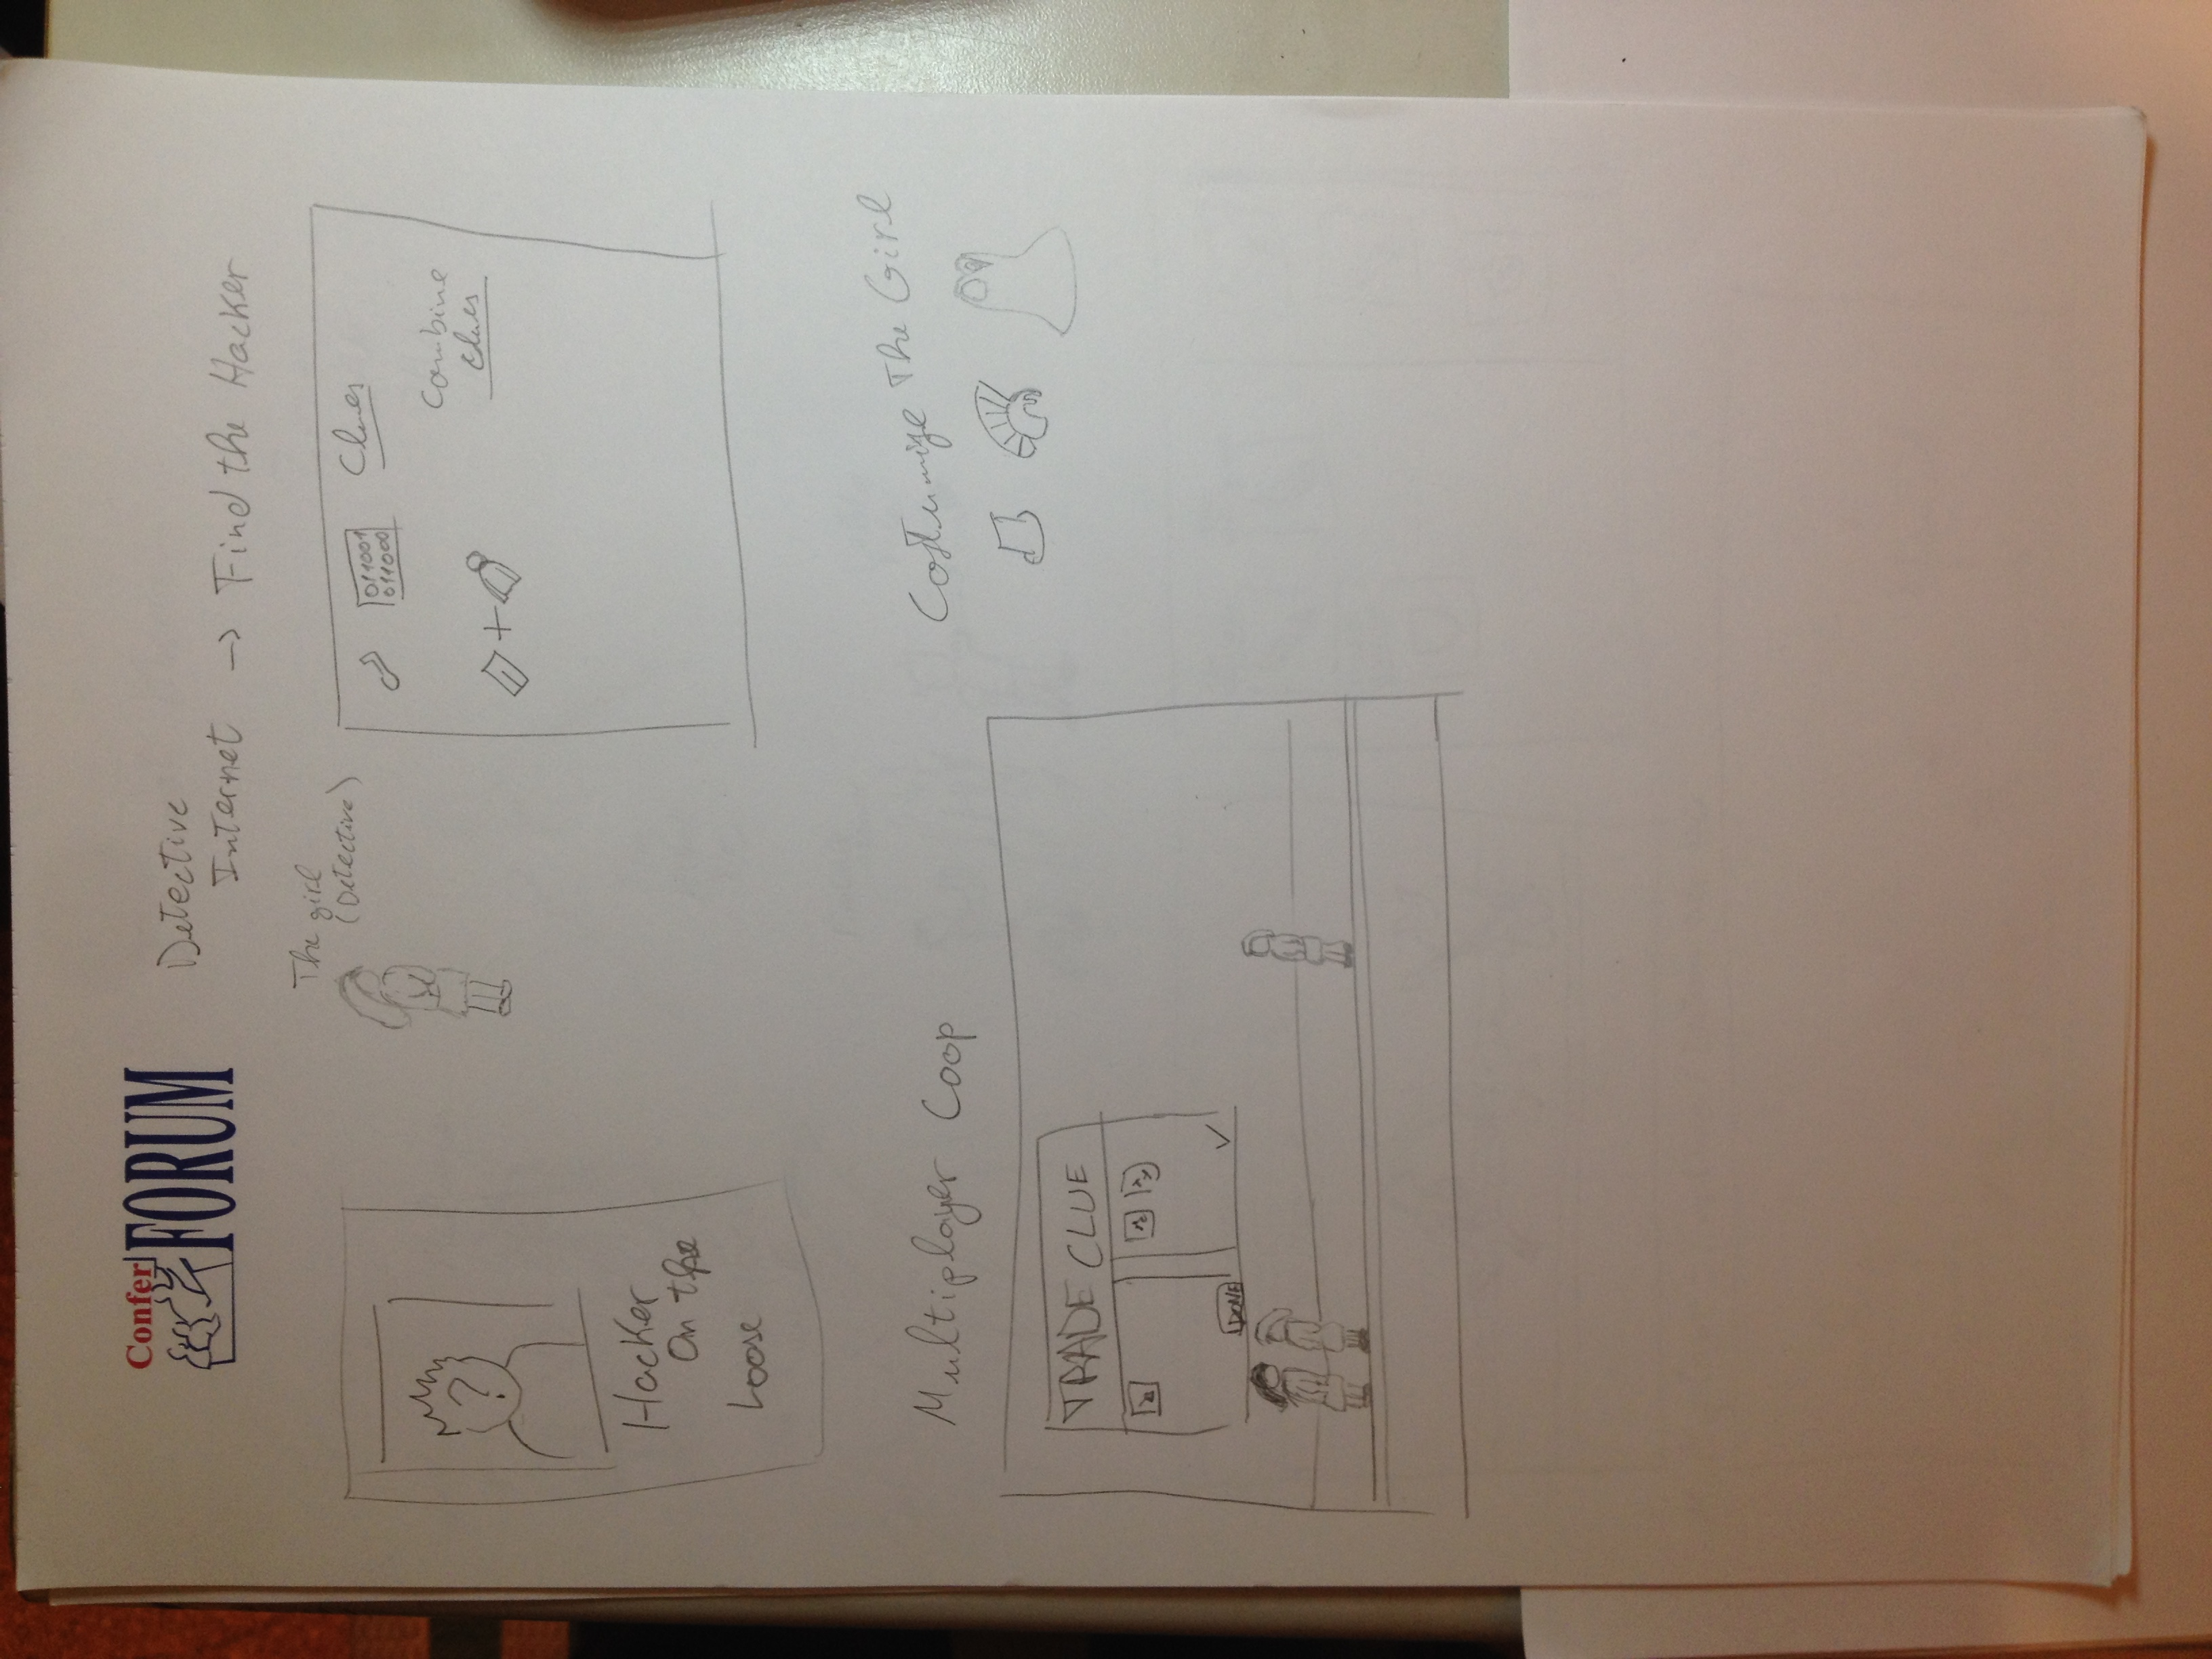
\includegraphics 
	[width = 0.75\textwidth , angle = 270] {Ricardo/ricardo_prototipo_3}
\caption{\label{att:fig:ric:prot3}} TerceiroProtótipo do Ricardo
\end{figure}

\begin{figure}[h]
\centering
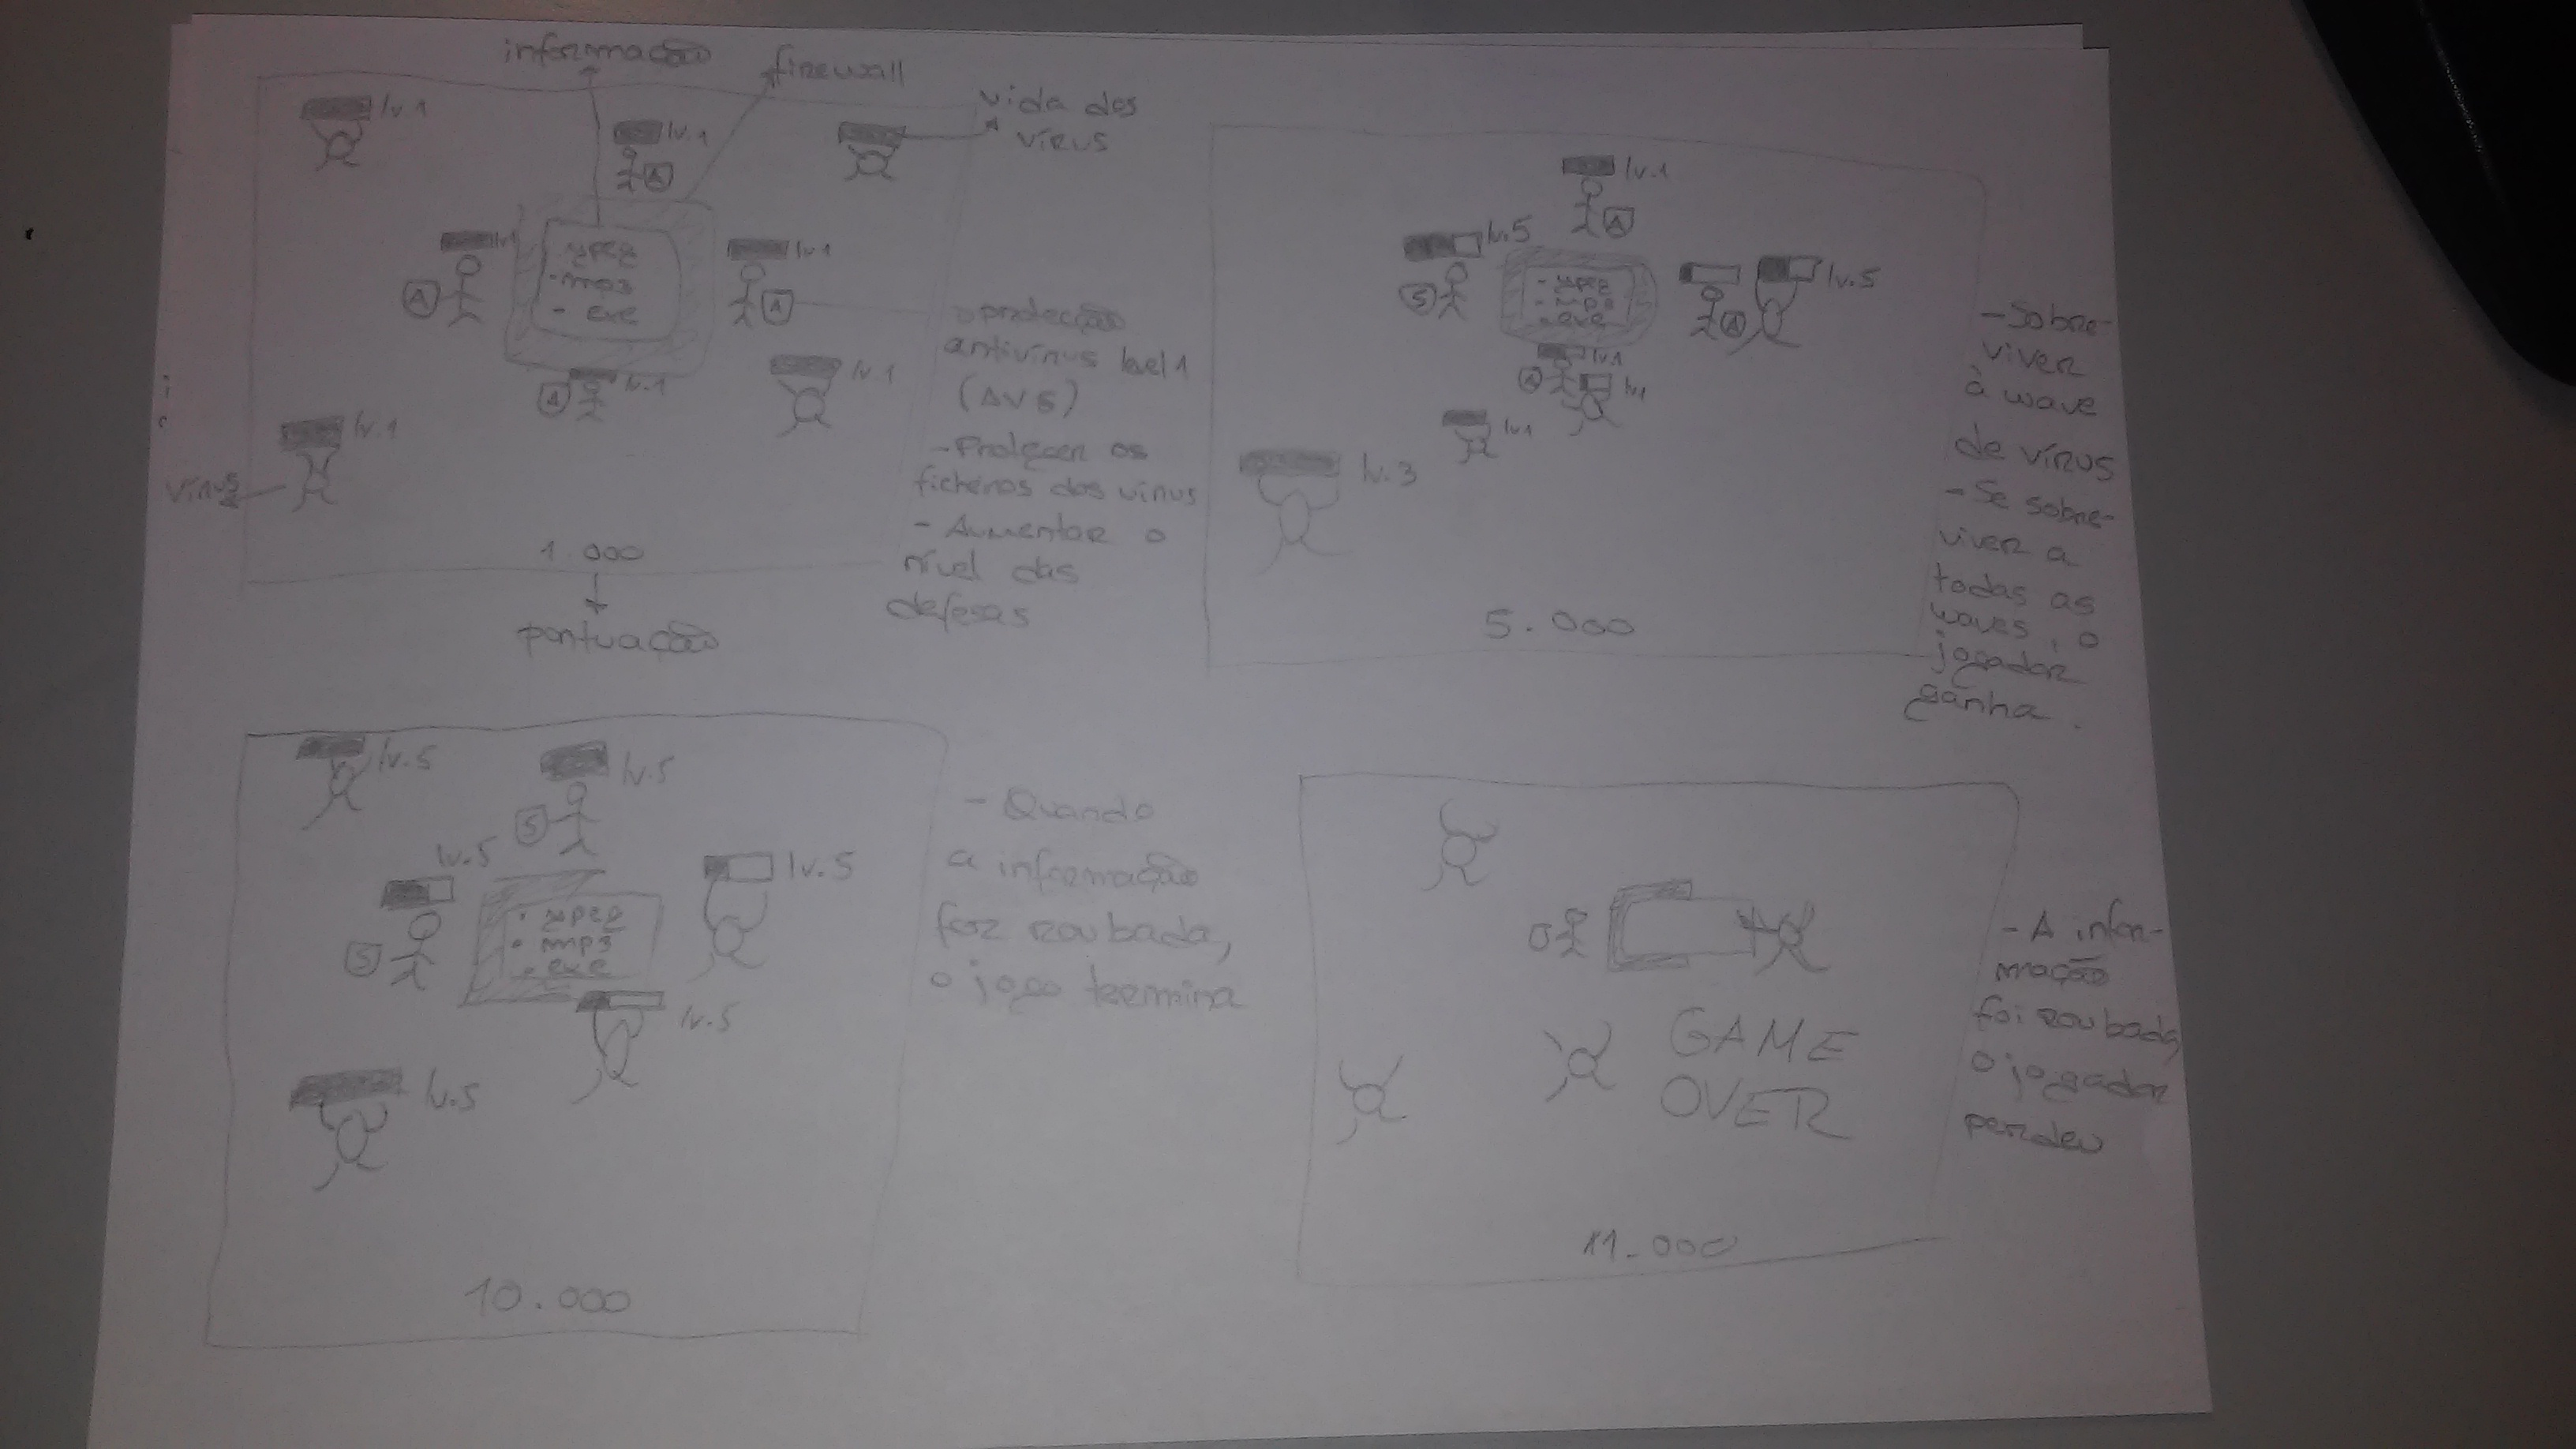
\includegraphics 
	[width = 0.75\textwidth] {Tiago/tiago_prototipo_1}
\caption{\label{att:fig:tiago:prot1}} Primeiro Protótipo do Tiago
\end{figure}

\begin{figure}[h]
\centering
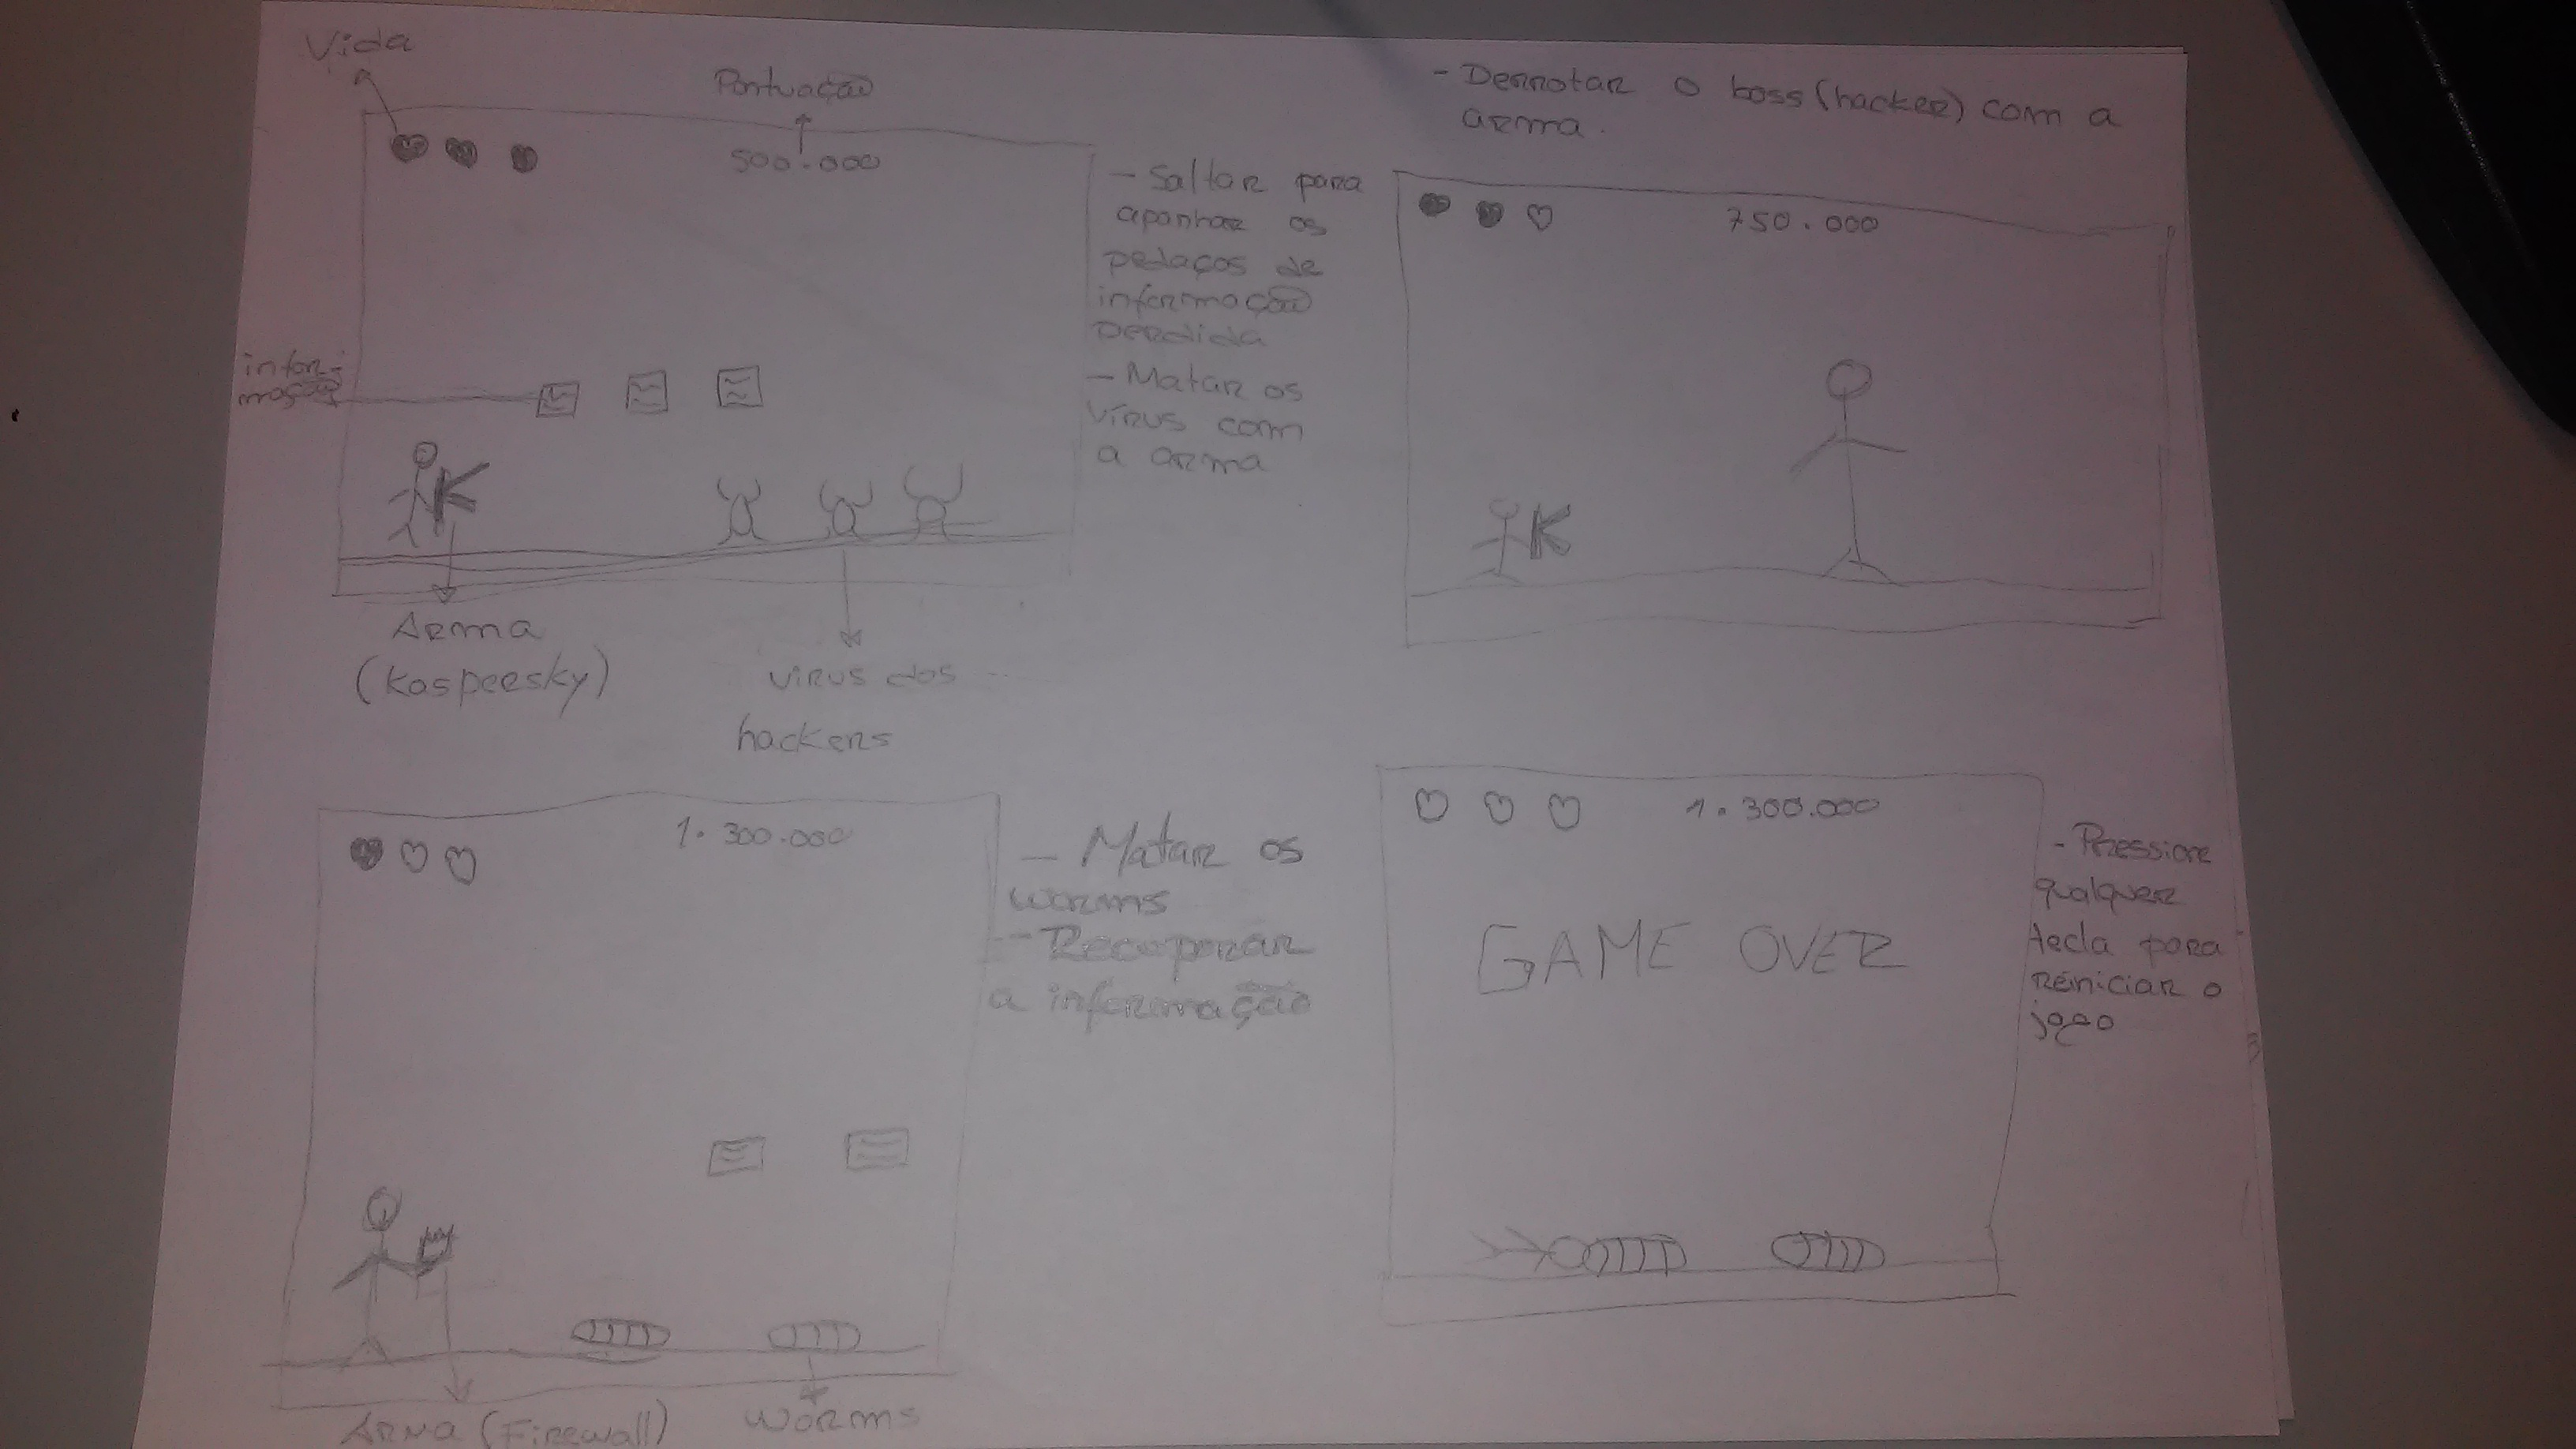
\includegraphics 
	[width = 0.75\textwidth] {Tiago/tiago_prototipo_2}
\caption{\label{att:fig:tiago:prot2}} Segundo Protótipo do Tiago
\end{figure}

\begin{figure}[h]
\centering
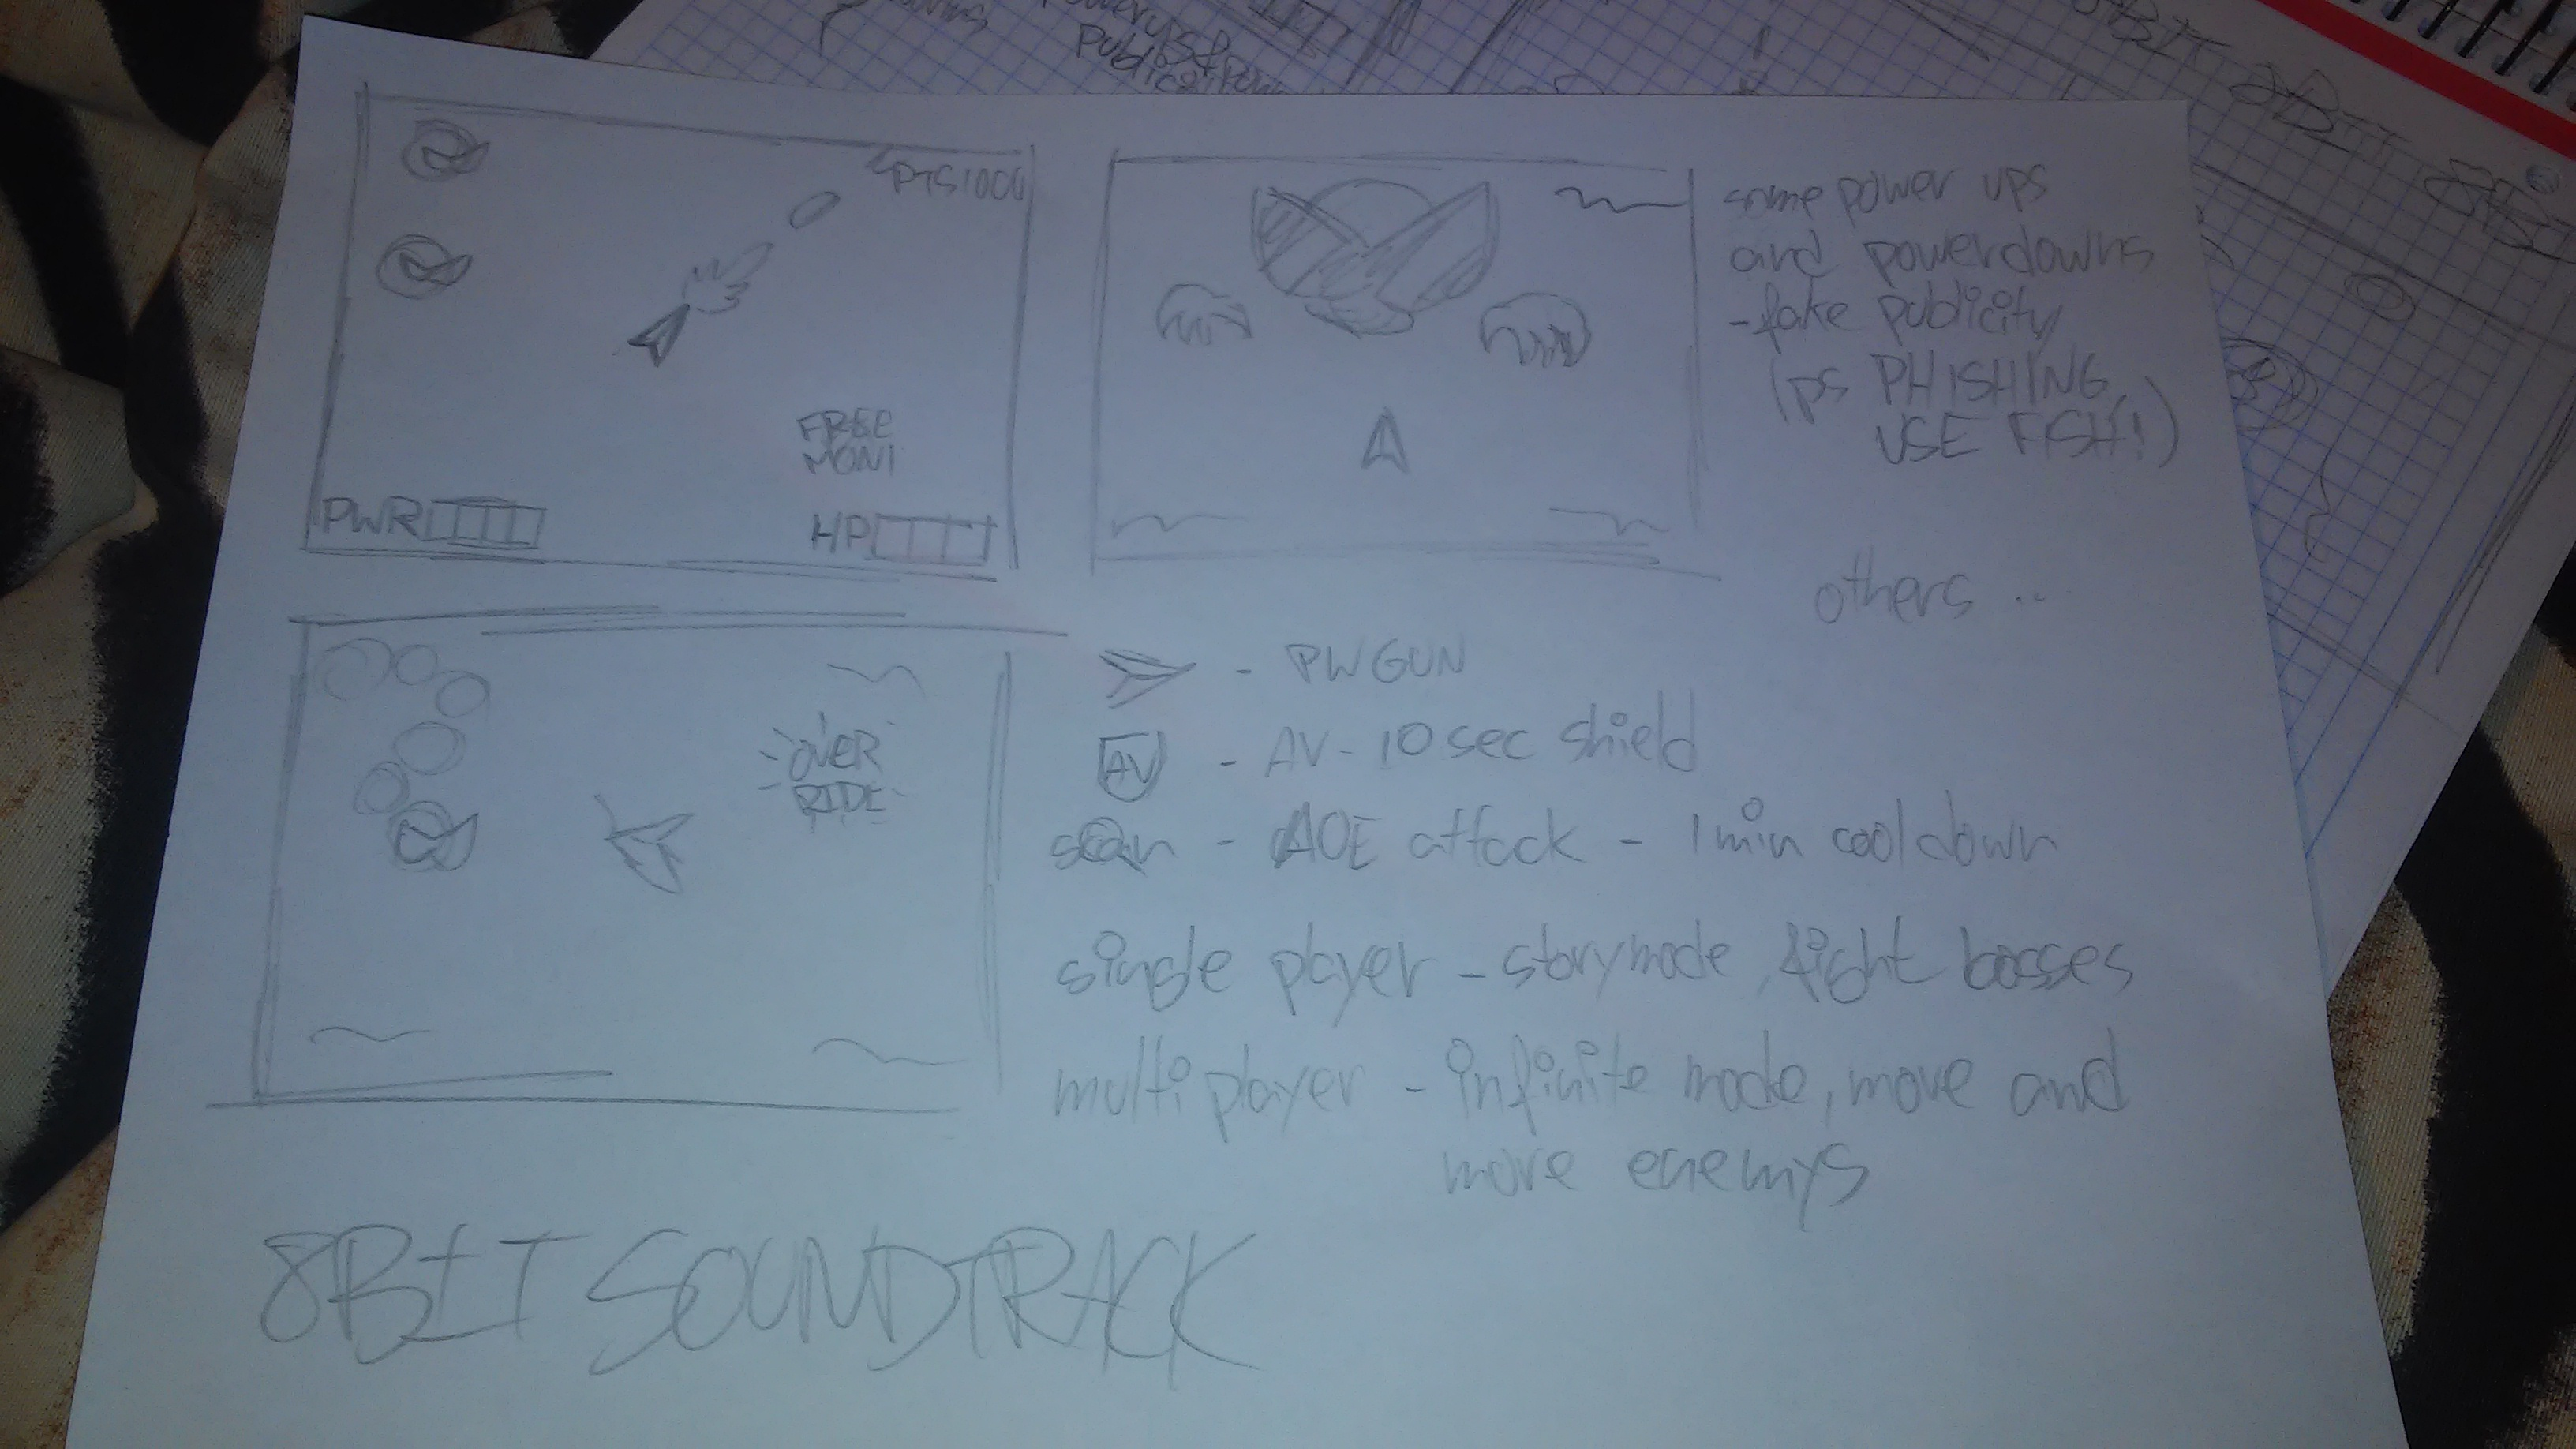
\includegraphics 
	[width = 0.75\textwidth] {Ian/ian_prototipo_1}
\caption{\label{att:fig:ian:prot1}} Primeiro Protótipo do Ian
\end{figure}

\begin{figure}[h]
\centering
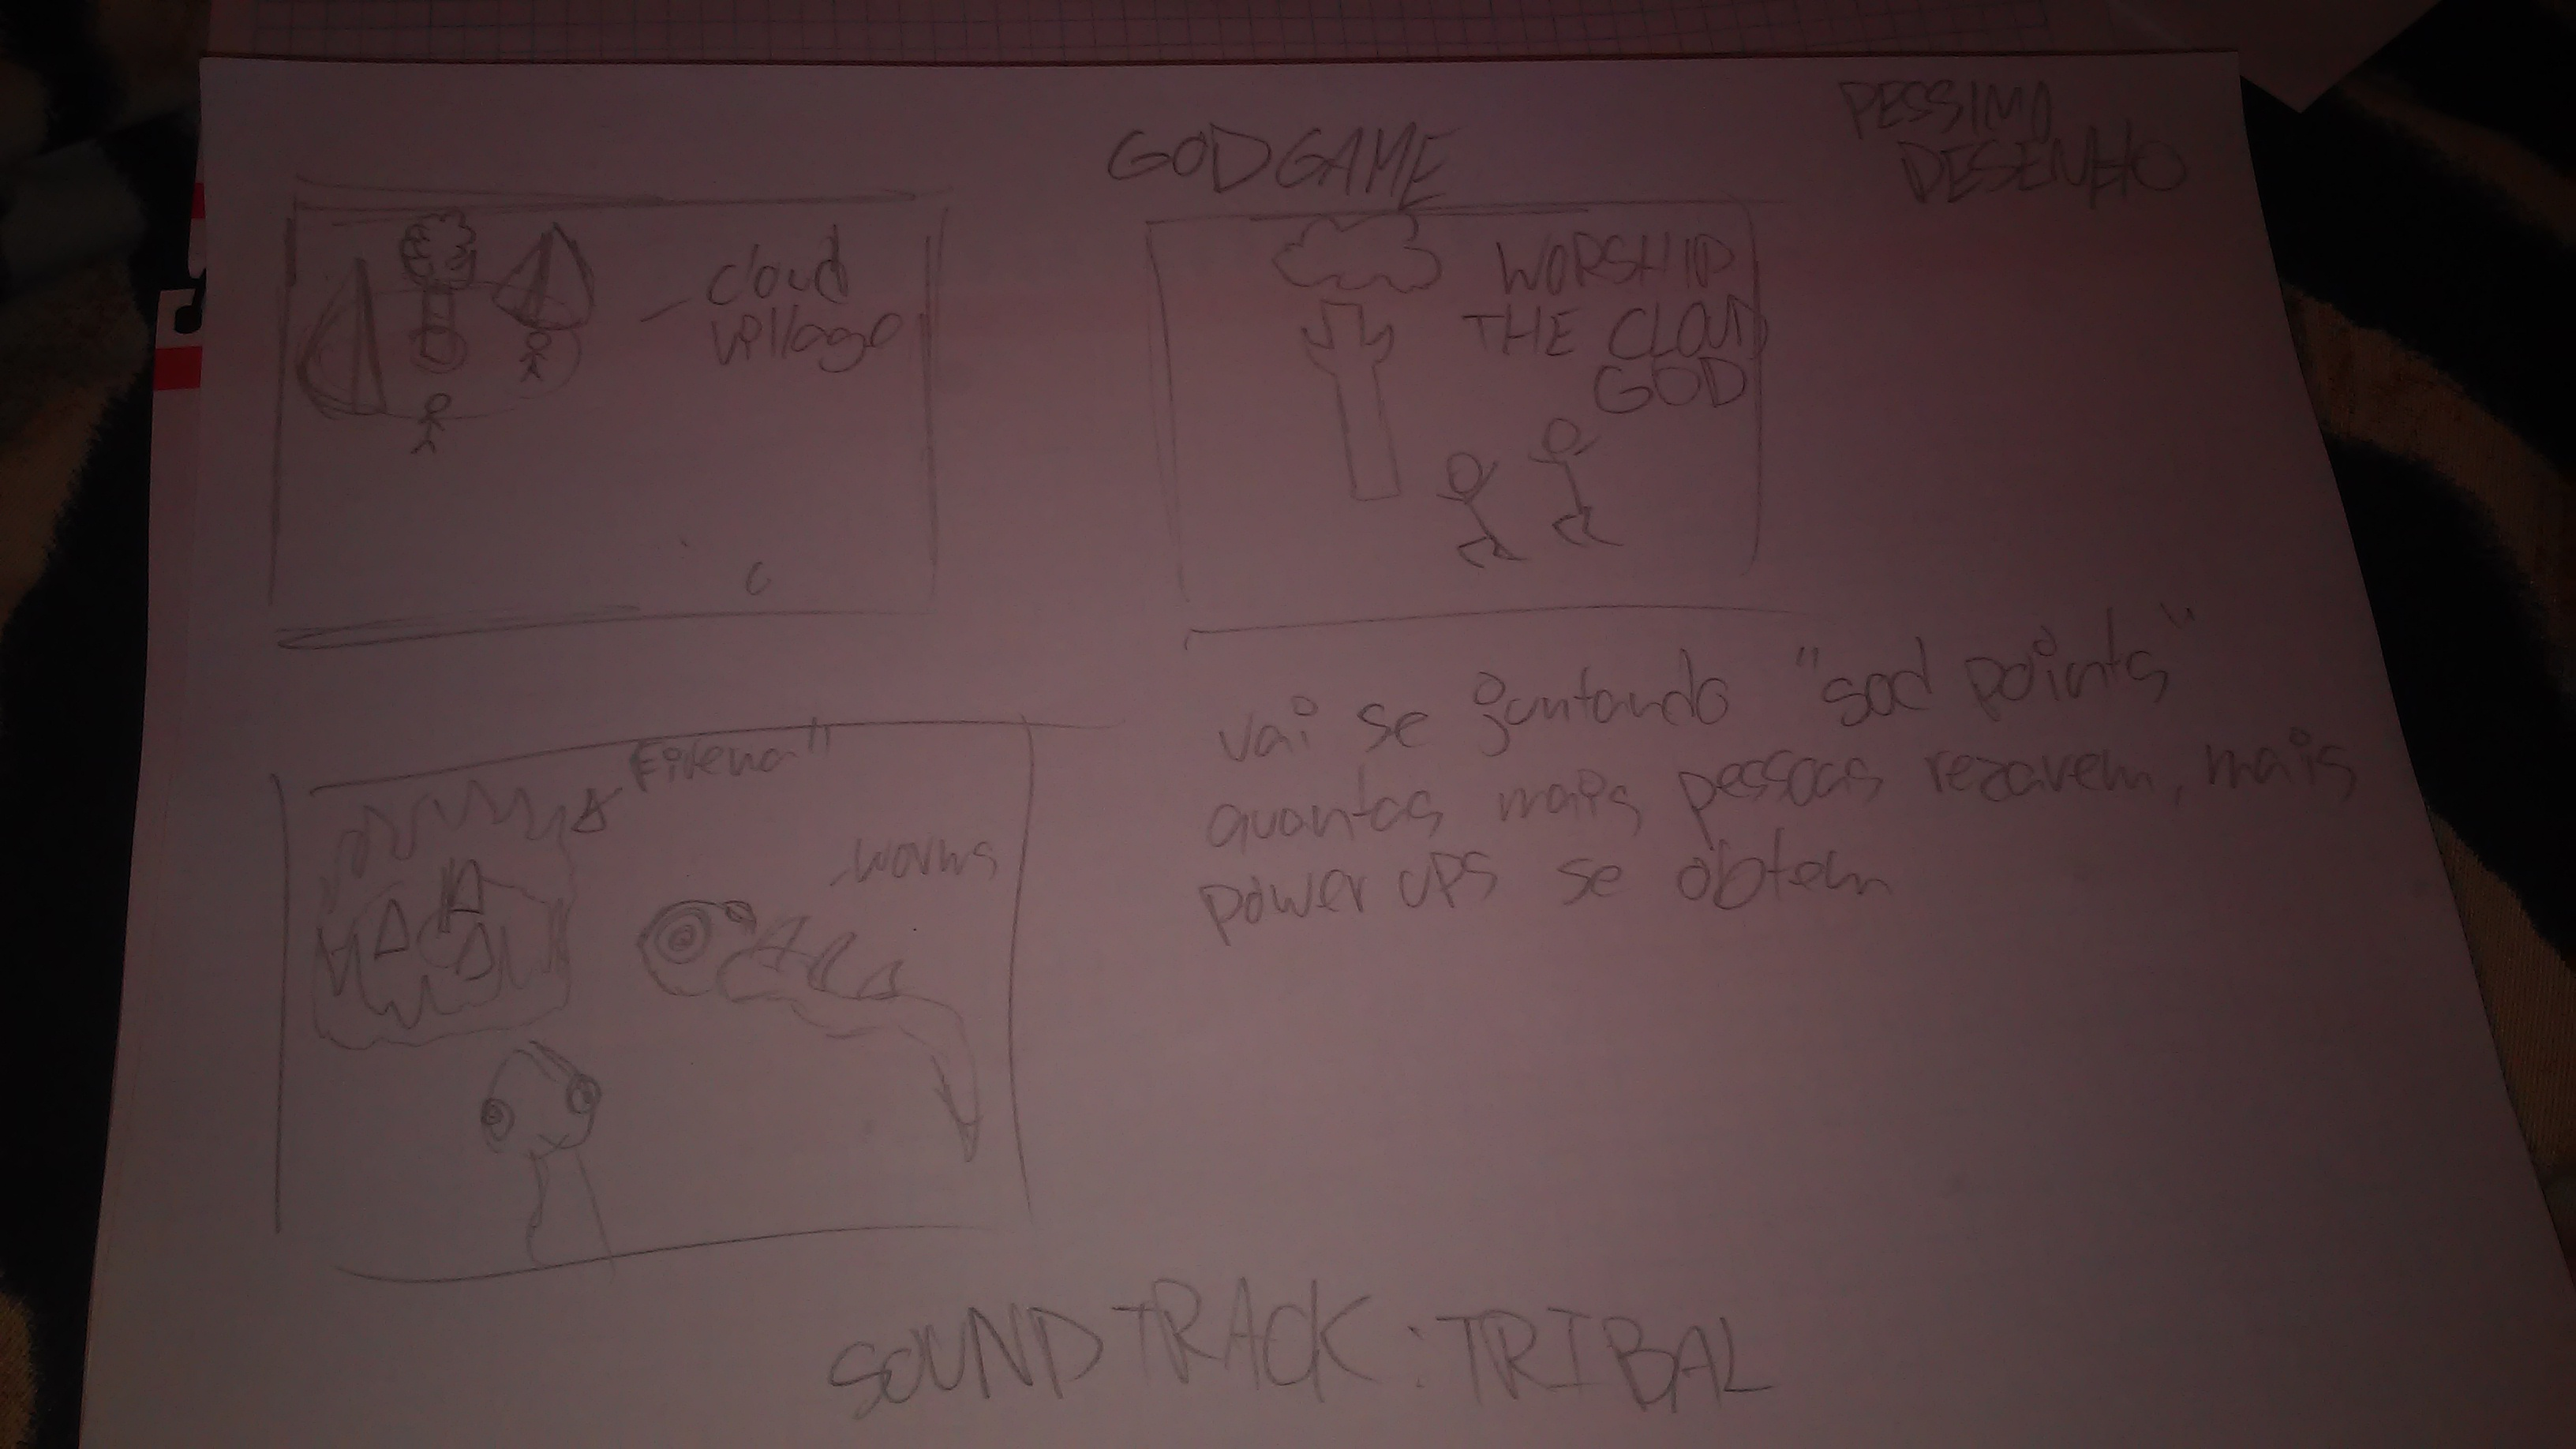
\includegraphics 
	[width = 0.75\textwidth] {Ian/ian_prototipo_2}
\caption{\label{att:fig:ian:prot2}} Segundo Protótipo do Ian
\end{figure}

\begin{figure}[h]
\centering
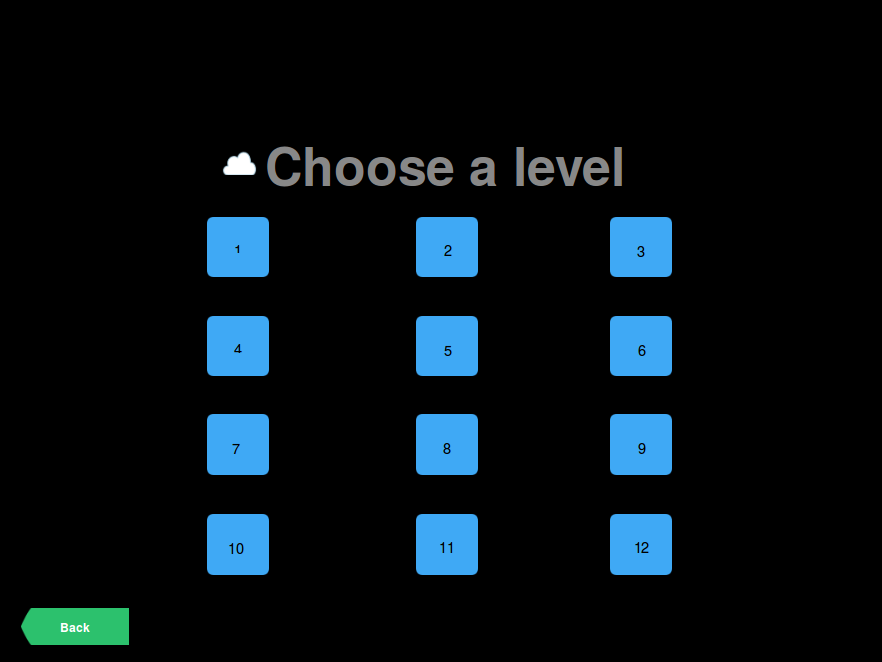
\includegraphics 
	[width = 0.65\textwidth] {FluiuiMenusPrototype}
\caption{\label{fig:fluidui}} Protótipo de Menus no FluidUI
\end{figure}

\begin{figure}[h]
\centering
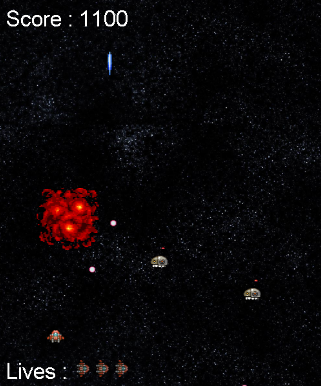
\includegraphics 
	[width = 0.65\textwidth] {PhaserGamePrototype}
\caption{\label{fig:phaser}} Protótipo de Jogo no Phaser
\end{figure}